\subsection{Casa integrante 1 - dataset $Red 1$} 

La entropía calculada fue de 0.049668, un valor bajo lo cuál indica que cada símbolo obtenido no arroja mucha información y es predecible.


\begin{figure}[H]\begin{center}
  \includegraphics[width=0.6\textwidth]{images/freq_ws_4_info.png}\vspace{1em}
  \caption{Frecuencias por protocolo}
\end{center}\end{figure}


\texttt{IPV4} (con 0.9955\%) fue el protocolo más escuchado en contraposición contra \texttt{ARP} (0.0019\%) e \texttt{IPV6} (0.0024\%), lo cuál tiene sentido por la naturaleza de estos últimos. Recordemos que ARP es un protocolo utilizado para encontrar la dirección MAC de un host a partir de su \texttt{IP} en la red y actualizar su tabla \texttt{ARP}. Esto sólo es necesario hacerlo cuando la tabla de un host no contiene una entrada para el host con el que quiere comunicarse. Si tenemos en cuenta la baja cantidad de dispositivos en la red es más que razonable obtener una tan baja presencia de \texttt{ARP}.

\begin{figure}[H]
    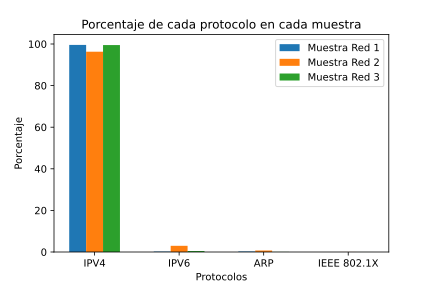
\includegraphics[scale=0.6]{images/resultados_generales/porcentaje_cada_protocolo_cada_muestra.png}\vspace{1em}
    \centering
    \caption{Porcentaje de cada protocolo en cada muestra capturada}
    \label{fig: porcentajes}
\end{figure}

Se pueden observar que el protocolo IPv4 domina las 3 redes, como es de esperarse. La red 2 


\begin{figure}[H]
    \centering
    \begin{subfigure}{0.45\linewidth}
        \includegraphics[scale=0.45]{images/resultados_diego/red_1_info.png}
        \caption{Red 1}
        \label{fig: info red 1}
    \end{subfigure}
    \begin{subfigure}{0.5\linewidth} 
        \includegraphics[scale=0.45]{images/resultados_agus/red_2_info.png}
        \caption{Red 2}
        \label{fig: info red 2}
    \end{subfigure}
    \begin{subfigure}{0.5\linewidth} 
        \centering
        \includegraphics[scale=0.45]{images/resultados_lion/red_3_info.png}
        \caption{Red 3}
        \label{fig: info red 3}
    \end{subfigure}
    \caption{Cantidad de información por cada símbolo en cada muestra.}
    \label{fig: informacion de los simbolos}
\end{figure}



Dado que la entropía es muy baja, la aparición de símbolos como \texttt{ARP} e \texttt{IPV6} aportan mucha información dada su escasa aparición.
\begin{figure}[H]
    \centering
    \begin{subfigure}[b]{0.3\textwidth}
        \centering
        \includegraphics[width=\textwidth]{images/resultados_diego/red_1_broadcast_unicast.png}
        \caption{Red 1}
        \label{fig: b/u red 1}
    \end{subfigure}
    \begin{subfigure}[b]{0.3\textwidth} 
        \centering
        \includegraphics[scale=0.7, width=\textwidth]{images/resultados_agus/red_2_broadcast_unicast.png}
        \caption{Red 2}
        \label{fig: b/u red 2}
    \end{subfigure}
    \begin{subfigure}[b]{0.3\textwidth} 
        \centering
        \includegraphics[width=\textwidth]{images/resultados_lion/red_3_broadcast_unicast.png}
        \caption{Red 3}
        \label{fig: b/u red 3}
    \end{subfigure}
    \caption{Proporción de Broadcast/Unicast en cada muestra.}
    \label{fig: informacion de los simbolos}
\end{figure}

\begin{table}[H]\begin{center}
  \begin{tabular}{|c|c|}
  \hline
  \textbf{Tráfico} & \textbf{Frecuencia} \\ \hline
  \texttt{Unicast   }&  0.998\%     \\ \hline
  \texttt{Broadcast      }&  0.0014\%     \\ \hline
  \end{tabular}
  \caption{Frecuencia de Unicast y Broadcast en la $Red 1$}
  \label{Red 1}
\end{center}\end{table}

\begin{table}[H]\begin{center}
  \begin{tabular}{|c|c|}
  \hline
  \textbf{Tráfico} & \textbf{Frecuencia} \\ \hline
  \texttt{Unicast   }&  0.9682\%     \\ \hline
  \texttt{Broadcast      }&  0.0317\%     \\ \hline
  \end{tabular}
  \caption{Frecuencia de Unicast y Broadcast en la $Red 2$}
  \label{Red 2}
\end{center}\end{table}

\begin{table}[H]\begin{center}
  \begin{tabular}{|c|c|}
  \hline
  \textbf{Tráfico} & \textbf{Frecuencia} \\ \hline
  \texttt{Unicast   }&  0.9862\%     \\ \hline
  \texttt{Broadcast      }&  0.0037\%     \\ \hline
  \end{tabular}
  \caption{Frecuencia de Unicast y Broadcast en la $Red 3$}
  \label{Red 3}
\end{center}\end{table}


La diferencia de porcentajes entre uno se debe a que \texttt{BROADCAST} es el tipo de tráfico de los paquetes ARP que por lo anterior vimos tienen bajas apariciones, mientras que UNICAST representa mayoritariamente todo el otro tráfico, por ejemplo, el que ocurrió durante el consumo de multimedia, que también por lo anterior, vimos eran los paquetes con mayor aparición.


\subsection{Casa integrante 2 - dataset $Red 2$}

• Porcentaje de tráfico Broadcast/Unicast sobre el tráfico total.

 - Broadcast: 756
 - Unicast: 23085


• Porcentaje de aparición de cada protocolo encontrado.

 - IPV4: 0.9629
 - ARP: 0.0297
 - IPV6: 0.0071
 - 34958: 0.0003
 
• Entropía de la red: 0.2572

• Cantidad de información de cada símbolo comparado con la entropía de la red.

 - IPV4: 0.0546
 - ARP: 5.0715
 - IPV6: 7.1318
 - 34958: 11.9562

\begin{table}[H]
\begin{center}
    \begin{tabular}{||c c||} 
        \hline
        Dataset & Entropía \\ [0.5ex] 
        \hline\hline
        $Red 1$ & $0.04966814662839276$ \\ 
        \hline
        $Red 2$ & $0.3494232951207893$ \\
        \hline
        $Red 3$ & $0.08226822373062319$ \\ [1ex] 
        \hline
    \end{tabular}
    \caption{Tabla de Entropía en las redes}
    \label{Tabla entropía}
\end{center}
\end{table}


\subsection{Fuente de información $S_{2}$ - Hosts distinguidos en la red } 
\subsubsection{Casa integrante 1 - dataset $Red 1$}

\begin{figure}[H]
    \centering
    \begin{subfigure}{0.5\linewidth} 
        \includegraphics[scale=0.5]{images/resultados_generales/red_1_info.png}
        \centering
        \caption{Red 1}
    \end{subfigure}
    \begin{subfigure}{0.5\linewidth} 
        \includegraphics[scale=0.5]{images/resultados_generales/red_2_info.png}
        \centering
        \caption{Red 2}
    \end{subfigure}
    \begin{subfigure}{0.5\linewidth} 
        \centering
        \includegraphics[scale=0.45]{images/resultados_generales/red_3_info.png}
        \caption{Red 3}
    \end{subfigure}
    \caption{Cantidad de información por cada símbolo en cada muestra.}
    \label{fig: informacion de los simbolos}
\end{figure}